%%%%%%%%%%%%%%%%%%%%%%%%%%%%%%%%%%%%%%%%%%%%%%%%%%%%%%%%%%%%%%%%%%%%%%%%%%%%%%%%
%2345678901234567890123456789012345678901234567890123456789012345678901234567890
%        1         2         3         4         5         6         7         8

\documentclass[letterpaper, 12 pt, conference]{ieeeconf}  % Comment this line out
                                                          % if you need a4paper
%\documentclass[a4paper, 10pt, conference]{ieeeconf}      % Use this line for a4
                                                          % paper

\IEEEoverridecommandlockouts                              % This command is only
                                                          % needed if you want to
                                                          % use the \thanks command
\overrideIEEEmargins
% See the \addtolength command later in the file to balance the column lengths
% on the last page of the document



% The following packages can be found on http:\\www.ctan.org
%\usepackage{graphics} % for pdf, bitmapped graphics files
%\usepackage{epsfig} % for postscript graphics files
%\usepackage{mathptmx} % assumes new font selection scheme installed
%\usepackage{times} % assumes new font selection scheme installed
%\usepackage{amsmath} % assumes amsmath package installed
%\usepackage{amssymb}  % assumes amsmath package installed

 \usepackage{array}
 \usepackage{amssymb}
 \usepackage{theorem}
 \usepackage{fancyvrb}%  extended verbatim environments
  \fvset{fontsize=\footnotesize,xleftmargin=2em}

\usepackage{graphicx,psfrag,pstricks,cite,amsmath,amssymb,latexsym}

\graphicspath{{./Figures/}}


\DeclareRobustCommand{\gumstix}{Gumstix\textsuperscript{\textregistered}}
\DeclareRobustCommand{\overo}{Overo\textsuperscript{\textregistered}}
\DeclareRobustCommand{\tobi}{Tobi~}
\DeclareRobustCommand{\pinto}{Pinto~}
\DeclareRobustCommand{\garmin}{Garmin\textsuperscript{TM}}
\DeclareRobustCommand{\houston}{Houston RADAR\textsuperscript{TM}}
\DeclareRobustCommand{\ICE_T}{\textcolor{Blue}{ICE-T}}
\DeclareRobustCommand{\UXAS}{\textcolor{Blue}{UxAS}}

\newtheorem{thm}{Theorem}[section]
\theoremstyle{definition}
\newtheorem{defn}[thm]{Definition}


\title{\LARGE \bf
Development and Flight Test of an Area Monitoring System Using Unmanned Aerial Vehicles and Unattended Ground Sensors 
}

%\author{ \parbox{3 in}{\centering Huibert Kwakernaak*
%         \thanks{*Use the $\backslash$thanks command to put information here}\\
%         Faculty of Electrical Engineering, Mathematics and Computer Science\\
%         University of Twente\\
%         7500 AE Enschede, The Netherlands\\
%         {\tt\small h.kwakernaak@autsubmit.com}}
%         \hspace*{ 0.5 in}
%         \parbox{3 in}{ \centering Pradeep Misra**
%         \thanks{**The footnote marks may be inserted manually}\\
%        Department of Electrical Engineering \\
%         Wright State University\\
%         Dayton, OH 45435, USA\\
%         {\tt\small pmisra@cs.wright.edu}}
%}

\author{Steven Rasmussen and Derek Kingston% <-this % stops a space
\thanks{This paper is based on work at the Air Force Research Laboratory's \emph{Control Science Center of Excellence}}% <-this % stops a space
\thanks{S. Rasmussen is a Principal Engineer for Miami Valley Aerospace LLC, Control Science Center of Excellence, Air Force Research Laboratory, Wright-Patterson AFB
        {\tt\small steven.rasmussen@wpafb.af.mil}}%
\thanks{D. Kingston is a Research Engineer with the Control Science Center of Excellence, Air Force Research Laboratory, Wright-Patterson AFB
        {\tt\small derek.kingston@us.af.mil}}%
}


\begin{document}



\maketitle
\thispagestyle{empty}
\pagestyle{empty}


%%%%%%%%%%%%%%%%%%%%%%%%%%%%%%%%%%%%%%%%%%%%%%%%%%%%%%%%%%%%%%%%%%%%%%%%%%%%%%%%%
\begin{abstract}
%
This document describes the motivation, theoretical description, development, and flight test of a system that utilizes unmanned air vehicles (UAVs) and unattended ground sensors (UGSs) to detect and image intruders on a road network. The need for completely autonomous behavior drives the design of this system so that the UAV makes onboard decisions based upon inputs from off-board sensors (unattended ground sensors). A complete road surveillance system consisting of a UAV and over 30 UGSs was designed and simulated. The system was also flight tested in a realistic operating environment.
%
\end{abstract}
%
%
%%%%%%%%%%%%%%%%%%%%%%%%%%%%%%%%%%%%%%%%%%%%%%%%%%%%%%%%%%%%%%%%%%%%%%%%%%%%%%%%%

\section{Introduction}
Research has been conducted for many years in the area of cooperative control of unmanned aerial vehicles (UAVs). The thrust of much of cooperative control research is to enable UAVs to work together to accomplish missions, thereby increasing mission performance and decreasing the number of humans required to control the system. However, many of those research results have not yet been integrated into battlefield systems. In order to reduce the number of humans involved, UAVs must be capable of performing tasks on their own, independent of human input. So, the question is \emph{`What can UAVs do on their own?'}.

In section \ref{sec:Autonomy} we propose that the answer to this question lies in the ability of the UAV to interpret sensed information and then act on it. To explore systems where multiple UAVs can sense the environment, make decisions, and implement those decisions, a type of sensor amenable to exploitation is required. As described in section \ref{sec:UGS}, an Unattended Ground Sensor (UGS) can be used in this manner. Using UGSs as off-board sensors, the UAVs can take sensor readings and then act on those readings\cite{kingston2012,krishnaCDC14,krishnaACC14}. In order to implement a complete UAV/UGS system a simulation was constructed (see section \ref{sec:Simulation}) and flight tests conducted (see section \ref{sec:FlightTest}).

\section{What UAVs Can Do Autonomously\label{sec:Autonomy}}
There has been a lot of research into creating teams of UAVs that can \emph{autonomously} cooperate to perform tasks\cite{Chandler:2001a,Richards:2002,Rasmussen:2004b,RasmussenShima:2007,ShimaSchumacher:2008,How:2009}. One unifying thread throughout this research is that the technologies that allow the UAVs to make decisions autonomously are either \emph{assumed} to exist or the tasks have been simplified to accommodate autonomous decision making. For instance, the algorithms in the articles \cite{Chandler:2001a,Rasmussen:2004b,RasmussenShima:2007,ShimaSchumacher:2008} assumed that \emph{automatic target recognition} (ATR) algorithms are available. In the article \cite{How:2009} UAVs detect and track targets, but to make the technology work in flight tests, different colored plaques were placed on top of the ground vehicles. Developing UAV systems that can perform tasks autonomously necessitates taking a step back and understanding what this means.

In order to accomplish a task autonomously, a UAV must have access to actionable sensed information. Actionable information refers to UAV-understandable data that the UAV can use to decide on the course of actions that it must perform to accomplish an assigned mission. The information must be sensed in order to make it possible for the UAV to get updated measurements for the task. Sensed information can be generated by sensors carried onboard the UAV or collected off-board and accessed via a communication device. Actionable information is generated from sensed information through the use of some kind of exploitation algorithm.

A number of different sensor modalities have been amenable to exploitation, to varying degrees of success, such as: radar for target tracking\cite{kingstonACC05}, acoustic sensors for gunshot location, and radio frequency sensors for locating radios and jammers\cite{wang2010jamming} . Visual sensors have been used, in a very limited way, for target tracking, but this requires a human to periodically update the target position in the image.

With the ability to collect actionable sensed information the UAV is able to take some measure of the environment, develop a plan to perform a desired task, and execute the plan using updates from the sensor, as feedback, during the task execution. 


\section{A Combined UAV/UGS System\label{sec:UGS}}
%One of the main obstacles to truly autonomous UAVs is the lack of reliable
%onboard sensing capability. 
If a UAV could identify and track objects of
interest independent of human operators, a wide variety of current surveillance missions
could be performed with minimal human oversight. However, given the immaturity
of such technology (especially with respect to visual sensors), we pose a
situation in which UAVs are combined with UGSs to create a system that attempts
to reduce the time a human operator needs to monitor UAV sensor feeds while
still providing valuable surveillance products. In a sentence, our goal is to research a
combined UAV/UGS system that detects intrusion on a road network and delivers
imagery of potential threats only when that imagery has a high likelihood of
containing an intruder.

Many current UGS systems are placed carefully and have line-of-sight to other
UGSs or to a ``gateway'' node. The main driver of these systems is very low
power so as to provide useful data for as long as possible without replacement.
Unfortunately, getting the collected data to a user can take
significant resources; often the gateway node has access to satellite
communication equipment and the alarms from the network of sensors
are routed back to operators via that communication link. This requires careful
setup and placement of the gateway node and usually requires a stable power
source (other than simply batteries). We propose a system with the main feature
that UAVs are used to query the UGSs. This would allow a higher density of UGSs
to be placed (as there would not be a need to connect to expensive,
hard-to-situate gateway nodes) as well as allow UGSs to be placed in areas with
difficult line-of-sight restrictions (sharp valleys and canyons).

In the most general sense, a system that combines UAVs and UGSs could operate
under a variety of circumstances and situations. However, in order to focus our
research efforts we will assume that intruders remain on the road network.

For a given road network, UGSs are placed strategically to increase the visibility of
movements of intruders. Although it is reasonable to imagine that such placement could
be optimized based on the structure of the road network, we begin our research with
the locations of the UGSs already determined. In practice, we place our UGSs based
on intelligence of enemy motion, locations that support improved sensor readings,
and ease of placement.

Our prototype unattended ground sensors record the time, position, speed, and direction 
of the intruder. Many currently available commercial UGS systems do not support all of these measurements,
however, it is reasonable that a small network of currently available
UGSs could determine all of these parameters. Theoretically, there is no
difference between querying a single UGS that determines this information and
querying in quick succession a small network of UGSs that records this level of
information. Each UGS has known, fixed position with characterized false alarm and
misdetection rates.

Note that each UGS operates completely independently and has no mechanism to report alarms to a
centralized base location. A UAV must query the UGS when in range to download
the stored intrusion detections. Based on that information, the UAV collects and stores onboard
relevant video clips for future delivery to a human operator for analysis. UAVs do not have any
sort of moving target indication or automated target tracking ability, so video clips are collected solely
based on the probability calculated from the combined sensor measurements uploaded to the UAV.

We concede that further research on UGS systems to extend their communication
range may obsolete the algorithms designed for this situation as communication
architecture is the primary feature that influences how UAV control decisions are made.


\section{Autonomous UAV/UGS Area Monitoring Development} \label{sec:hardware}
In order to implement an effective UAV/UGS monitoring system, both software and hardware components were designed, implemented, tested, and fielded. While some of the software, such as that for the ground control station, had been developed in other programs, all of the software in the final system was either modified or developed during the construction of this area monitoring system. Multiple software components interacted via a set of messages that were defined and updated iteratively over the course of two years of development. By the end of flight testing, the software had reached version 17. Major hardware challenges included constructing and integrating a computer on-board the UAV that was capable of performing the necessary computations, data storage, and networking; and design and implementation of an UGS capable of generating and storing intruder alerts and then transferring them to the UAV.

\subsection{UAV On-Board Processor}
Because of it's small size, processing capability, and the ability to integrate it into our design, we choose the \overo ~family of embedded processors\cite{gumstixwebsite} to act as both the on-board and UGS computers. Each of \overo~ includes an ARM processor, micro-SD card reader, 256 or 512 Mb memory, and run an embedded version of Linux. The operating system, application programs, and boot code were loaded on to 16 Gb micro-SD cards, which were used for booting the operating system, running the applications, and data storage. On-board the UAV, the \tobi expansion board was used to break out necessary signals as well as provide USB and Ethernet interfaces. The \tobi was attached to a custom integrated circuit board that was designed to be an interface between the \tobi breakout board and the autopilot. Wi-Fi communications were provided using a USB Wi-Fi dongle connected to the \tobi. See Figure \ref{fig:OnBoardProcessorLayout} for a diagram of the on-board processor components.

Similar to~\cite{li2009multiple}, the on-board processor interfaces to an autopilot that handles all the flight-critical aspects of operation. Using the native autopilot datalink, the onboard processor can ``pass-through'' messages directly to the ground station control station allowing the operator to maintain visibility of the onboard decisions being carried out. The onboard package includes a wifi communications link that enables communication with UGSs and dismount operators in the field (using wifi-enabled tablets). Additionally, the UAV carries a video digitizer which the onboard computer uses to enable recording and storage of video collected by the aircraft electro-optical gimbaled sensors.

\begin{figure}[htb]
\centering
      \includegraphics[width=0.45\textwidth]{OnBoardProcessorLayout}
      \caption{On-Board processor hardware diagram.}
      \label{fig:OnBoardProcessorLayout}
\end{figure}

\subsection{UGS Design/Operation}
Our initial design of the system included a purchase of already existing UGSs, but after discussing our requirements with many UGS manufactures we could not find UGS that could locally store alerts and ultimately transfer them directly to the UAV. All of the UGS systems that we found consisted of sensors that immediately communicated alerts to nodes where they were processed and sent to operators via line-of-site or satellite links. While it would have been possible to modify these nodes to store alerts and send them to the UAV, it would have been very costly to field these systems in the number we anticipated. We decided that developing our own UGS would give us the flexibility needed for research access, as well as being more cost effective.

Our UGS design consisted of a custom circuit board, a GPS receiver, a Doppler radar, a Wi-Fi module, and an \overo~ module. The UGS board is designed to integrate the other components using their factory provided connectors as well as facilitate power saving by allowing power switching for the Wi-Fi and GPS components. A Houston SS300 Doppler radar\cite{houstonradar} acts as the intruder sensor. It returns speeds for moving objects in its field of view and range. While the GPS receiver reports the position of the UGS, it also reports the GPS time which allows synchronization of alerts over all of the UGS and UAVs. The \overo retrieved GPS and radar inputs, generated and stored filtered intruder alerts, and sent them to the UAV when it was in range. See Figure \ref{fig:UgsHardwareLayout} for a photograph of the UGS and a diagram of the UGS components.

\begin{figure}[htb]
\centering
      \includegraphics[width=0.45\textwidth]{UgsHardwareLayout}
      \caption{UGS hardware diagram.}
      \label{fig:UgsHardwareLayout}
\end{figure}

\subsection{UAV/UGS Communication}
In order to communicate with the UGS and transfer recorded measurements, a message interface was developed. Table \ref{fig:ACCA_IUGS_MESSAGE_PASSING} lists the messages passed between the UAV and the UGS when the UAV flies close enough to the UGS to establish a Wi-Fi connection. During the mission, the UAV periodically sends a \textit{HeartbeatMessage} that contains its network address to any available UGS or UAV in Wi-Fi range. Reception of a \textit{HeartbeatMessage} causes the receiver to connect as a client to the enclosed address and send back a heartbeat response. When the sending UAV receives a \textit{HeartbeatResponse}, it sends a message asking for any intruder alerts since the time the two entities previously communicated. The receiver sends the requested \textit{IntruderAlerts}, if any are available, and a \textit{QueryResponse} that lists all of the alerts sent. Each message received, except the \textit{HeartbeatMessage}, is acknowledged by sending a \textit{VicsAck} message.
\begin{table}
\caption{UAV/UGS message passing.}
\label{fig:ACCA_IUGS_MESSAGE_PASSING}
\begin{center}
\begin{tabular}{|m{1.0cm}|m{1.0cm}|m{4.8cm}|}\hline
 \textbf{FROM}  & \textbf{TO}     & \textbf{MESSAGE}\\ \hline \hline
UAV & UGS & \emph{HeartbeatMessage} - Send Heartbeat over multicast channel.\\ \hline
UGS & UAV & \emph{HeartbeatResponse} - Send response to heartbeat message as TCP/IP client\\ \hline
UAV & UGS & \emph{MessageQuery} - Ask for all messages since last contact.\\ \hline
UGS & UAV & \emph{QueryResponse} - Send list of all messages being sent.\\ \hline
UGS & UAV & \emph{IntruderAlert, DismountMessage} - send all messages that match the query.\\ \hline
UAV & UGS & \emph{VicsAck} - Send an acknowledgement for each message received.\\ \hline
\end{tabular}
\end{center}
\end{table}


\section{ICE-T Autonomous UAV/UGS Area Monitoring Architecture}
The hardware and communication described in section~\ref{sec:hardware} forms the heart of the overall UAV/UGS system, however, a tremendous amount of supporting systems were also needed for successful deployment and test. As a part of the Value of Information in Collaborative Systems (VICS) initiative, members of the Air Force Research Laboratory (AFRL) on the Intelligent Control and Evaluation of Teams (ICE-T) program and the Human Effectiveness Directorate (RH) designed, implemented, and tested a system comprised of Unmanned Aerial Vehicles (UAVs) and Unattended Ground Sensors (UGS) that performs autonomous intruder detection and isolation over a given area. It was necessary to: design a common message set; develop on-board processing capability; design and manufacture UGS; and integrate with the human operator interface Vigilant Spirit Control Station (VSCS). Figure \ref{fig:AreaMonitoringArchitecture} is a system overview of how the various elements of the system fit together.


\begin{figure*}[thb]
\centering
      \includegraphics[width=0.9\textwidth]{AreaMonitoringArchitecture}
      \caption{Area Monitoring Architecture}
      \label{fig:AreaMonitoringArchitecture}
\end{figure*}


The major groupings in Figure \ref{fig:AreaMonitoringArchitecture} are Ground Station, PCC, Piccolo, On-Board Processor, UGS, and Dismount. Elements in the Ground Station group facilitate integration of the system with a human operator. The Piccolo Command Center (PCC) is the ground control station provided by the autopilot manufacturer. Piccolo is the autopilot on the UAV. All software elements of the On-Board Processor are implemented using an \overo~ module. The UGS group represent all UGS that are deployed. Provision was made for human interaction with the UGS, represented by the group labeled Dismount.

\subsection{Messages}
Elements of the system are coordinated using three Light Weight Message Protocol (LMCP) Message Data Modules (MDM) marked CMASI, ICET, and VICS in the diagram. CMASI was designed to be a generic message set for communication with cooperative control algorithms.
%, see Table \ref{fig:SELECTED_CMASI_MESSAGES} for a sample of these messages.\\
ICET messages add commands to implement ICE-T generated tasks. The VICS message set was designed specifically for the UAV/UGS monitoring system and contains UGS/Intruder Isolation messages.
%, see Table \ref{fig:SELECTED_VICS_MESSAGES}.
A fourth message set, provided by the autopilot manufacturer, is used to communicate with the Piccolo autopilot. VSCS uses an additional message set, CMF, to communicate with the UAV.

%\begin{table}
%%\begin{center}
%\caption{Selected CMASI messages.}
%\label{fig:SELECTED_CMASI_MESSAGES}
%\begin{tabular}{|m{3.0cm}|m{4.8cm}|}\hline
%\emph{AirVehicleConfiguration} & Provides information regarding a vehicle's configuration items.  \\ \hline
%\emph{AirVehicleState} &  Provides basic information regarding the vehicle state with regard to its location and orientation in the world, and current velocity in body axis.
% \\ \hline
%\emph{AutomationRequest} &  This is the primary message for requesting action from the automation service. \\ \hline
%\emph{KeepInZone} & Describes the outer boundary of operations for the entire UAV team or a subset of the vehicle team. \\ \hline
%\emph{KeepOutZone} & Defines a keep-out zone. This describes a volume where vehicles are not allowed to fly.  \\ \hline
%\emph{LineSearchTask} & Defines a line search task. A line search is a list of points that forms a polyline.  \\ \hline
%\emph{MissionCommand} &  A mission to be performed by a vehicle. This sends a new list of waypoints to an aircraft and commands the aircraft to start flying the mission starting at the specified "FirstWaypoint".  \\ \hline
%\emph{VehicleActionCommand} & A message that specifies actions that should be performed by the specified aircraft. \\ \hline
%\emph{Waypoint} & A simple waypoint class for vehicle routing  \\ \hline
%\end{tabular}
%%\end{center}
%\end{table}
%
%
%
%\begin{table}
%%\begin{center}
%\caption{Selected VICS messages.}
%\label{fig:SELECTED_VICS_MESSAGES}
%\begin{tabular}{|m{2.6cm}|m{5.3cm}|}\hline
%\emph{CommTransferTask} & Request UAV to visit a location, establish connection and handshake all non-payload messages\\ \hline
%\emph{ImageLineSearchTask} & Overloads the line search task to include options for image data gathering \\ \hline
%\emph{IntruderAlert} & Occurs when a UGS detects an object. \\ \hline
%\emph{PatrolTask} & Patrol task for establishing constant circuit visit to a set of locations \\ \hline
%\emph{RadarEnableMessage} & Allow dismount to selectively enable or disable radar  \\ \hline
%\emph{UgsLaydown} & Combined road nework and fixed UGS locations \\ \hline
%\emph{UgsManagementTask} & Persistent super-task for managing sub-tasks related to patrol, isolation, capture and delivery.  \\ \hline
%\end{tabular}
%%\end{center}
%\end{table}


\subsection{Ground Station}
The VSCS is the center of ground station activities. Using VSCS the operator monitors the state of the mission and can send UAV commands via the Piccolo Vehicle Specific Module (PVSM) or send high level task commands via the Ground Cooperative Control Algorithms (GCCA). The PVSM interfaces with the Piccolo Command Center (PCC) and translates between the CMF and Piccolo message sets. The VSCS receives vehicle state updates and sends vehicle commands via the PVSM. When sending tasks and receiving mission updates, the VSCS communicates to the GCCA using LMCP messages. The GCCA acts as buffer between the VSCS and the Airborne Cooperative Control Algorithms (ACCA) by interpreting requests from VSCS and requesting messages from the ACCA. The GCCA sends LMCP messages to the Ground Vehicle Specific Module (GVSM) which interfaces with the PCC to send/receive the message over the Piccolo pass-through channel.

\subsection{PCC}
For the demonstration system, the PCC is used as a safety ground station and to pass messages to the Piccolo autopilot. A safety operator uses the PCC to facilitate launching and landing the UAV, and can take control of the UAV during the mission if needed for safety. For message passing, the PCC can send autopilot commands to the autopilot, or LMCP messages on a pass-through channel. Messages sent on the pass-through channel are forwarded to the On-Board Processor group.

\subsection{Piccolo}
The Piccolo group contains the Piccolo autopilot. The Piccolo autopilot implements plan following, guidance, stability and control, on-board the UAV. It also acts as a pass-through conduit for messages sent from the Ground Station to the On-Board Processor. New plans/vehicle commands can be sent from the PCC or the On-Board Processor. Note that ICE-T UAVs use either Piccolo or Kestrel autopilots. The Kestrel autopilot is integrated into the system in a manner similar to the Piccolo.

\subsection{On-Board Processor}
The On-Board Processor group represents software running on-board the UAV. Functions of the on-board software include: mission planning, task management, and vehicle management. The Airborne Cooperative Control Algorithm (ACCA) accepts messages that define: tasks, flight boundaries, air vehicle configuration, air vehicle states, and mission requests. These messages are used to construct plans for the UAV to conduct the mission. Mission plans are forwarded to the Piccolo through the Airborne Vehicle Specific Module (AVSM), which translates between LMCP and Piccolo messages. As the UAV perform the mission plan, the ACCA monitors the state of the mission, sends sensor pointing commands, and updates the plans as necessary.
The road surveillance algorithms execute as tasks in the ACCA. Each task starts with a mission request from the VSCS and continues until superseded by a new mission request. The UGS patrol algorithm generates a set of communication transfers tasks, centered on the UGSs, that are integrated into a waypoint plan which is sent to the Piccolo. As the UAV flies the plan, it performs communication transfer tasks at each of the UGS. During the transfer task, each UGS sends the UAV any intruder alerts that it collected. If there has been an intruder, the controller can plan new routes to visit other UGSs in order to capture an image or video clip of the intruder.

\subsection{Dismount}
Human (dismount) interaction with the UGS was facilitated by supporting messages such as interchanging text, image, and sound files between the dismount and the UGS. In this manner, an operator in the field with a Wi-Fi enabled tablet could connect to an overhead UAV and give it commands or learn about the status of nearby UGSs.


\section{Simulating UAV/UGS Scenarios\label{sec:Simulation}}
The AMASE simulation is used to simulate the UAV/UGS scenarios, see Figure \ref{fig:AMASE_UAV_UGS_Simulation_Snapshot}. AMASE was developed by members of AFRL's Aerospace Vehicles Technology Assessment \& Simulation Branch (AVTAS) to provide a common framework for research and development of cooperative control algorithms \cite{DuquetteMST:2009}. AMASE was extended for this project in order to simulate \emph{communications}, \emph{on-board data processing}, and \emph{UGS}. AMASE includes the capability to connect to external programs using TCP/IP connections and a message protocol called CMASI \cite{Duquette:2010}. CMASI was developed by AFRL researchers to allow communication between cooperative control algorithms, ground stations, and simulations.
%Figure \ref{fig:UAV_UGS_SimulationArchitecture} diagrams the various components and connections used in this simulation.

Extensive simulation testing significantly improved the software development time. The ability to interface the exact code running onboard the aircraft to the simulation allowed numerous corner cases to be fully tested. When fielding a system comprised of so many distributed hardware and software elements, it is hard to over-emphasize the value of simulation testing.

\begin{figure}[htb]
\centering
      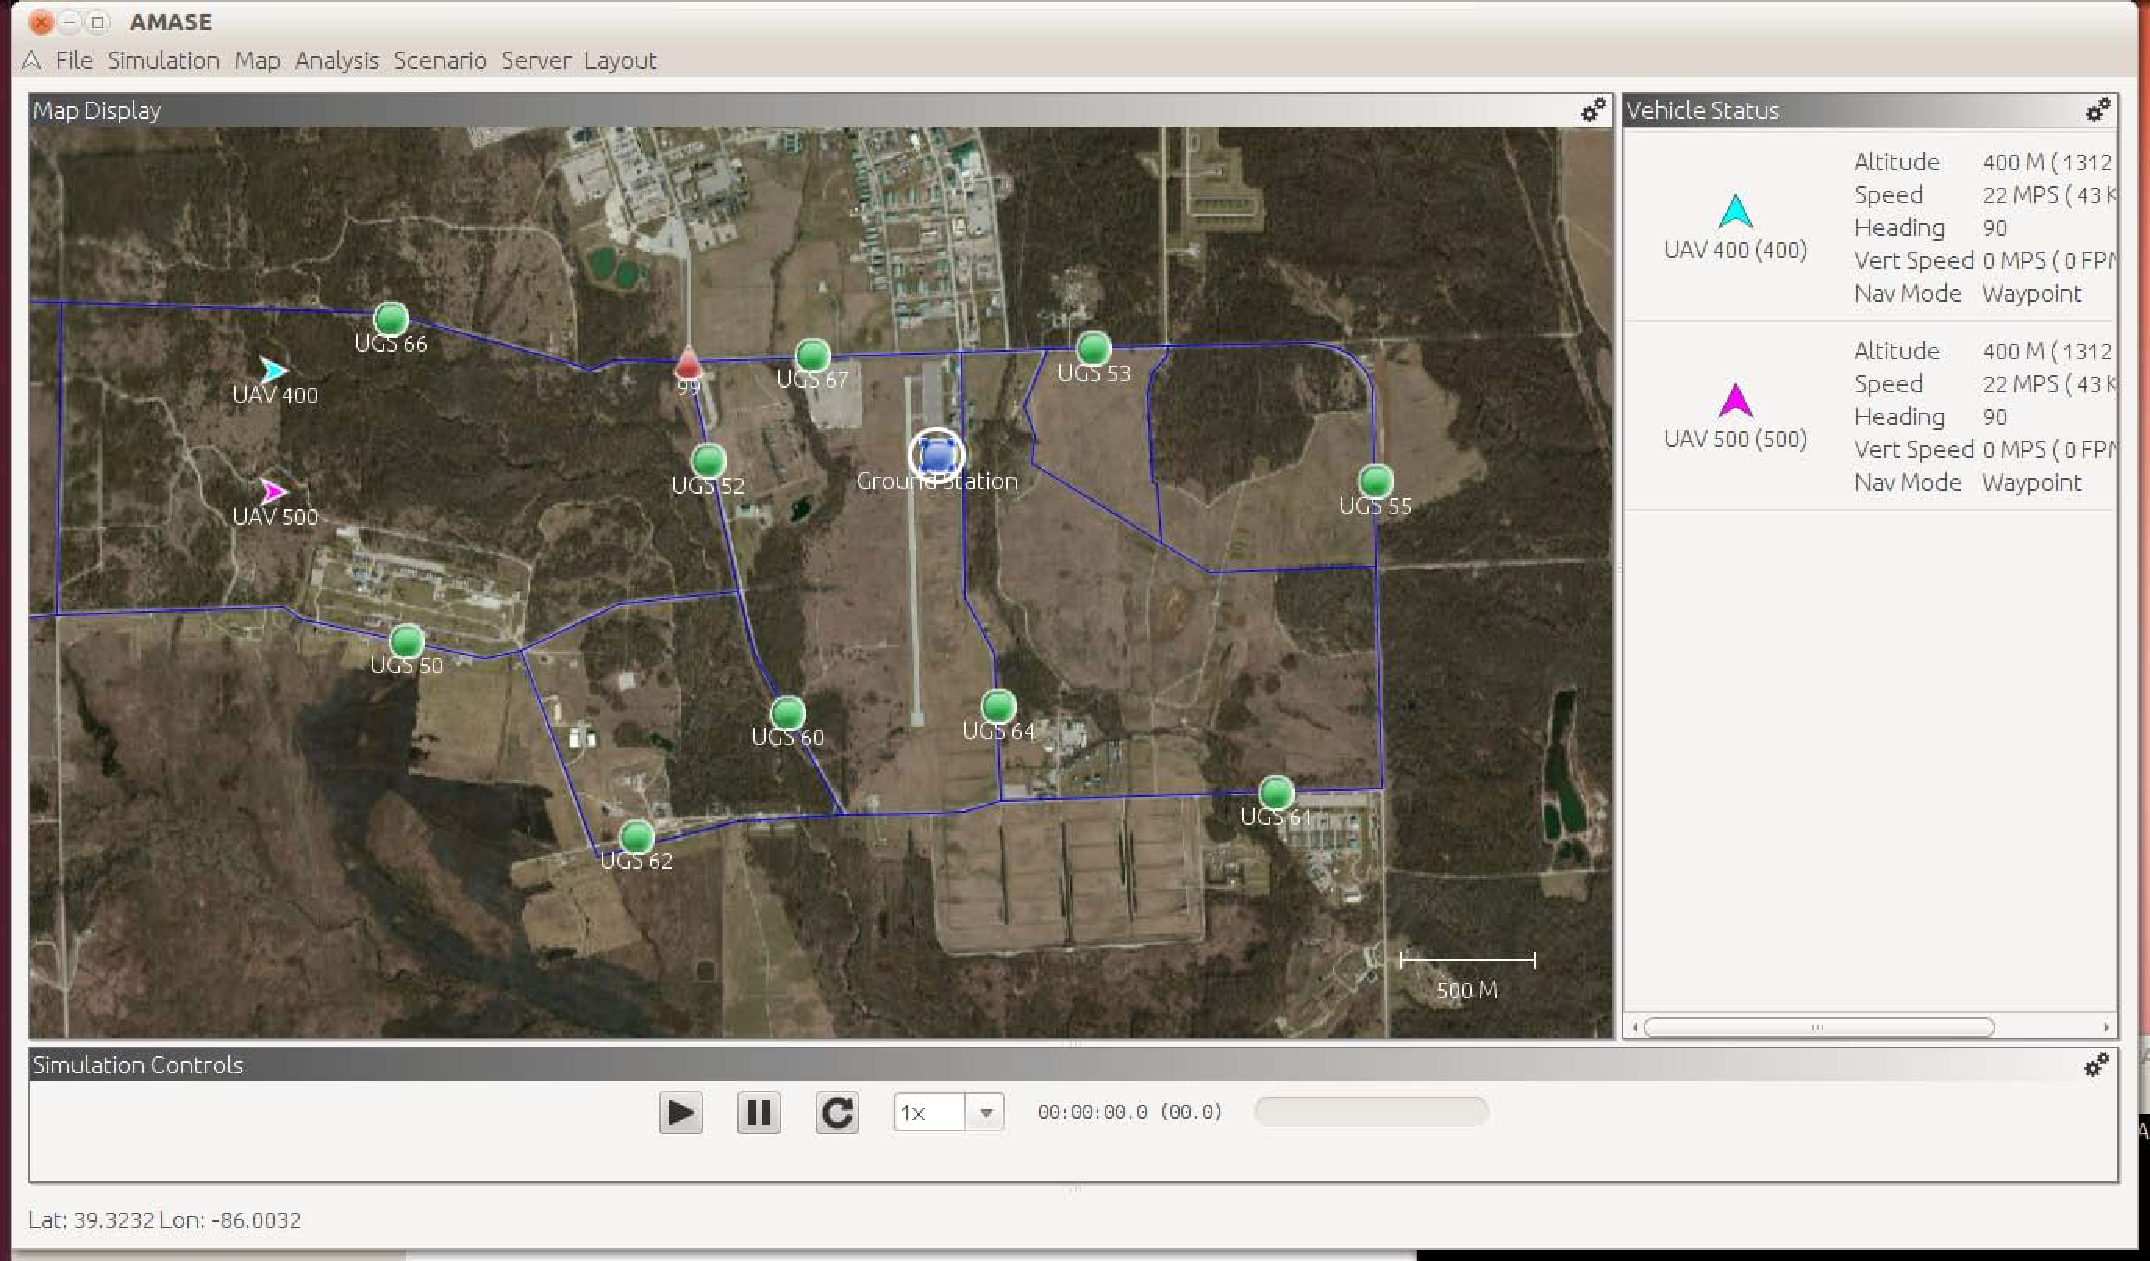
\includegraphics[width=0.45\textwidth]{AMASE_UGS_Scenario}
      \caption{AMASE UAV/UGS Simulation Snapshot}
      \label{fig:AMASE_UAV_UGS_Simulation_Snapshot}
\end{figure}

%\begin{figure}[htb]
%\centering
%      \includegraphics[width=0.5\textwidth]{AMASE_UGS_Diagram}
%      \caption{UAV/UGS Simulation Architecture}
%      \label{fig:UAV_UGS_SimulationArchitecture}
%\end{figure}



\section{Flight Testing/Demonstration\label{sec:FlightTest}}
In order to demonstrate the ability of this system to monitor an area of roads, it was necessary to demonstrate it in realistic scenarios. To accomplish this, all of the sub-systems were iteratively designed and flight tested and the full system was flight demonstrated. During the final test, over 30 UGSs were placed along roads of the test range. Each UGS was powered by a large battery cell that enabled them to collect information for two weeks. When airspace was available, the UGSs were visited by one of our gas-powered UAVs (up to 8 hour endurance) which used the collected information to record standard and infrared imagery of potential intruders.

\subsection{Sub-system Flight Tests}
Communication availability is the critical element for system operation. Due to the complex interaction of radios, UAVs, antennas, and operating environments, the only reliable method to determine the effect of communications on the system was to exercise it during actual flights. The two communication links that needed to be tested were the UAV-To-GCS and the UAV-To-UGS Wi-Fi.  The other major element that it was necessary to test in flight was the onboard processor and its interaction with the autopilot.

\subsubsection{UAV-To-GCS}  We assumed that the UAV-To-GCS would be adequate to transfer required messages from the UAV to the GCS. For the system demonstration, this link was part of the Piccolo autopilot radio link. It is controlled by the autopilot and shares the radio bandwidth with the critical autopilot commands. We found that the throughput on this link was much lower than we expected and care must be taken to choose which messages to transfer to the GCS. 
\subsubsection{UAV-To-UGS} The UAV-To-UGS link is implemented using Wi-Fi radios. Various configurations of this link were tested many times, both air-to-ground and ground-to-ground. We found that we had to disable the analog video transmitter on the UAV because it interfered with the range of Wi-Fi even though each was on a separate frequency channel. After many flight tests, we established that communicate from the UAV to the UGS could reliably be established when in a 0.5km range.
\subsubsection{Onboard to Autopilot} The onboard processor was designed to control the actions of the UAV by sending plans and commands to the autopilot. This can be tested on the ground in a hardware-in-the-loop simulation, but to ensure safe operations, it must also be flight tested in a controlled manner. One concern is that the onboard process could overload the autopilot or send harmful commands. This set of tests ensured that processor stayed within its limits as well as showed that the safety operator could disable the onboard processor at any time.

\subsection{Flight Demonstration and Data Collection}
In order to demonstrate its capabilities and collect data from a realistic scenario, the Road Monitoring system was deployed in a large \emph{Force-on-Force} military exercise, over a two week period. The exercise took place in an unimproved wooded region with dirt and gravel roads that covered a 35 km by 60 km area. There were many military type vehicles as well as ground troops. Because of the large number of vehicles moving on the roads, our algorithms designed for single intruders were not suitable, but other elements of the system could be exercised and valuable information/experience could be obtained by distributing the UGS throughout the exercise area.  

\subsubsection{On-Board Plan Generation and Execution}
When intruders were determined to be on certain segments of the road network, a request for imaging that road segment was sent directly to the UAV for processing. The onboard processor utilized accurate road locations to generate waypoints and camera steering commands and send them directly to the autopilot. The method for building the waypoints and camera steering commands is described in~\cite{kingstonSPIE09}. With the sensor steering automated, the onboard processor could begin recording digitized video of the road segment under surveillance. Later, the collected video would be downloaded and interpreted by human operators. The ``hands-off'' road monitoring provided by this capability was well received by operators as it offloads the normally tedious task of manually maintaining sensor view of the road.



\subsubsection{UGS Data Collection}
Thirty-one UGS were deployed on roads in the exercise area, see Figures \ref{fig:AllUgs} and \ref{fig:UGSPlacementForFlightTests}. Because of the size of the area and the ruggedness of the terrain, it took a couple of long days to place the UGS and initialize them. Once the UGS were in place, they were left, collecting data, until the end of the two-week-long exercise. Most of the UGS continued collecting data until they were retrieved after the exercise, but there were two that failed early.\\\\
Over the two weeks, the set of UGSs generated 53,000 intruder alerts. Many intruder alerts were false alarms and were attributed to sensitivity of the sensor to phenomena such as moving trees and rain. Because the UGS used the GPS receiver to precisely synchronize their clocks, the times that intruder alerts were generated can be used to compare alerts from different UGS. Since the UGS locations are known, distances between the UGS were calculated and used, along with the alert times and measured speeds, to calculate arrival windows for intruder at down-stream UGS. If alerts were found at the downstream UGS in the arrival window, they were paired with the alerts from the upstream UGS in a track. Figure \ref{fig:UGS_Tracks30MinWindow_01} shows an example of tracks generated over a 30 minute time window.  Alerts that were included in tracks were assumed to be true alerts. In this manner all of the intruder alerts were examined and it was found that about 30\% of the intruder alerts were true and 70\% were false alarms. 

\subsubsection{Retrieving Data from the UGS with a UAV}
During the exercise, the UAVs were directed to fly over the UGS to collect intruder alerts either using operator selected waypoints from the PCC or by using the on-board software to generate plans, see Figures \ref{fig:UgsPatrolPlan} and \ref{fig:UgsMonitoringPath}. Over the course of the exercise the UAVs collected 4300 intruder alerts from UGS, or roughly 8\% of the alerts generated. There were two issues that caused this number to be lower that it could have been, flight restrictions and data bandwidth.\\\\
During the exercise, the airspace was managed by military controllers who were responsible for safe operation of manned and unmanned aircraft. The airspace was managed by imposing restrictions on flight altitudes and areas. Because of these flight restrictions, the UAVs could only occasionally visit many of the UGS, and were never able to visit some of the UGS.\\\\
The other issue was the data bandwidth available from the UAV to the ground. For an intruder alert to be retrieved from an UGS and delivered to the operator, it is transferred between the elements on the thick green line in Figure \ref{fig:AreaMonitoringArchitecture}. The transfer starts at the IUGS block and then goes through: ACCA, PA, PCC, GVSM, GCCA, to the GCS block. The data bandwidth bottleneck is the connection between the autopilot and the PCC. This is the Piccolo pass-through connection, which shares the same radio as the command-and-control link for the Piccolo autopilot. The ACCA automatically transferred all intruder alerts to the autopilot for download to the GCS. Because of the pass-through limitation, the UGS were configured to upload alerts to the ACCA that were generated within the preceding hour, reducing the number of alerts collected by the UAV. Ultimately, only 240 alerts were transferred to the GCS. 



\begin{figure}[htb]
\centering
      \includegraphics[width=0.46\textwidth]{AllUgs}
      \caption{All of the UGS constructed for the exercise.}
      \label{fig:AllUgs}
\end{figure}

\begin{figure}[htb]
\centering
      \includegraphics[width=0.46\textwidth]{UgsPlacement_02a}
      \caption{UGS Placement for flight tests.}
      \label{fig:UGSPlacementForFlightTests}
\end{figure}

\begin{figure}[htb]
\centering
      \includegraphics[width=0.46\textwidth]{UGS_Tracks30MinWindow_01}
      \caption{Intruder alert tracks for a 30 minute time window.}
      \label{fig:UGS_Tracks30MinWindow_01}
\end{figure}

\begin{figure}[htb]
\centering
      \includegraphics[width=0.46\textwidth]{UgsMonitoringPath_02}
      \caption{UGS patrol flight path, based on operator selected waypoints.}
      \label{fig:UgsMonitoringPath}
\end{figure}

\begin{figure}[htb]
\centering
      \includegraphics[width=0.46\textwidth]{UgsPatrolPlan}
      \caption{UGS patrol plan, generated on-board the UAV.}
      \label{fig:UgsPatrolPlan}
\end{figure}

\begin{figure}[htb]
\centering
      \includegraphics[width=0.46\textwidth]{RoadSearchPlans_02}
      \caption{UAV road search plans, generated on-board the UAV.}
      \label{fig:RoadSearchPlans}
\end{figure}

\subsubsection{Lessons Learned}
% comms: difficulty, unreliability, limited --> value of onboard processing
% airspace integration
% false alarm rate, high numbers of intruders

The purpose of testing the combined UAV/UGS surveillance system in a realistic environment was to determine which concepts are applicable and useful in such an environment and also to determine assumptions that led to degradation of system usefulness.

The most prominent feature in realistic operating environments and especially in a multi-autonomous-entity system is that of communications reliability. Without exception, assumptions on the availability, reliability, and bandwidth of the communication channels impacted design and ultimate system usefulness. It is paramount to recognize during the design phase that autonomous entities must be able to operate with limited or absent communication and must be programmed to handle communication failure. Reasonable failsafes, re-tries, and time-outs must all be carefully designed and tested to ensure the system is robust to communication failure. By augmenting the autopilot with onboard decision making, working around the inevitable communication loss is possible. We plan to increase the ability of the UAV to make complex decisions onboard as that feature directly enables communication-robust operation.

Testing autonomous systems in complex, human-dominated domains causes numerous integration challenges. Of particular note, airspace restrictions and availability frequently impacted the way in which missions could unfold. It may be useful to think of autonomous agents actively pursing onboard decisions in a limited, geo-fenced area, but in reality, a complex, changing airspace forces careful consideration of movements of UAVs. Future systems that integrate with air tasking and consider it during planning will have much greater applicability and acceptance.

Finally, a primary hinderance to any completely autonomous system is the quality of the sensors available for determining actionable information. Our motivation for eschewing onboard target recognition stems from an awareness that such processes often contain high false alarm rates leading to very poor system behavior. However, the UGSs in our scenario also had high false alarm rate. Although the UGS information did directly impact the subsequent surveillance tasks, sifting through the high numbers of intruders and false alarms could not reliably be done autonomously. In the future, we plan to reduce the sensitivity of the UGS to external phenomena (raising the mis-detection rate in order to improve the false alarm rate) as well as autonomously reason on high numbers of intruders and likely false alarms.

\section{Future Work}
Flight test results indicated that utilizing an onboard processor to direct UAVs in high-level decision making provides tremendous utility. Our future plans include expanding the capability of the onboard decision making by exploring collaborative control of multiple UAVs working together to track down single intruders. In parallel, we recognize that the current UAV/UGS system has numerous deficiencies that should be addressed. In particular, improving the false alarm rate of the individual sensors (by reducing their sensitivity) and considering estimation of multiple simultaneous intruders.

\section{Conclusions}
This article described the development and flight test of a system that utilizes unmanned air vehicles and unattended ground sensors to detect and image intruders on a road network. Test of the system in a two-week realistic situation showed that the system has validity and applicability. However, careful consideration of communication limitations, airspace integration, and sensor false alarm rate are key to successful future operations. A primary component that enables communication-degraded operation is the onboard processor which augments the autopilot and provides high-level reasoning on the information pertinent to the mission.

\bibliographystyle{IEEEtran}
\bibliography{IEEEabrv,ICUAS2015}



%\section{INTRODUCTION}
%
%Your goal is to simulate, as closely as possible, the usual appearance of typeset
% papers. This document provides an example of the desired layout and contains
% information regarding desktop publishing format, type sizes, and type faces.
%
%\subsection{Full-Size Camera-Ready (CR) Copy}
%
%If you have desktop publishing facilities, (the use of a computer to aid
% in the assembly of words and illustrations on pages) prepare your CR paper
%  in full-size format, on paper 21.6 x 27.9 cm (8.5 x 11 in or 51 x 66 picas).
%  It must be output on a printer (e.g., laser printer) having 300 dots/in, or
%  better, resolution. Lesser quality printers, such as dot matrix printers,
%   are not acceptable, as the manuscript will not reproduce the desired quality.
%
%\subsubsection{Typefaces and Sizes:} There are many different typefaces and a large
%variety of fonts (a complete set of characters in the same typeface, style,
% and size). Please use a proportional serif typeface such as Times Roman,
% or Dutch. If these are not available to you, use the closest typeface you
%  can. The minimum typesize for the body of the text is 10 point. The minimum
%  size for applications like table captions, footnotes, and text subscripts
%  is 8 point. As an aid in gauging type size, 1 point is about 0.35 mm (1/72in).
%   Examples are as follows:
%
%\subsubsection{Format:} In formatting your original 8.5" x 11" page, set top and
%bottom margins to 25 mm (1 in or 6 picas), and left and right margins
%to about 18 mm (0.7 in or 4 picas). The column width is 88 mm (3.5 in or 21 picas).
% The space between the two columns is 5 mm(0.2 in or 1 pica). Paragraph
% indentation is about 3.5 mm (0.14 in or 1 pica). Left- and right-justify your
% columns. Cut A4 papers to 28 cm. Use either one or two spaces between sections,
% and between text and tables or figures, to adjust the column length.
%  On the last page of your paper, try to adjust the lengths of the
%  two-columns so that they are the same. Use automatic hyphenation and
%   check spelling. Either digitize or paste your figures.
%
%\begin{table}
%\caption{An Example of a Table}
%\label{table_example}
%\begin{center}
%\begin{tabular}{|c||c|}
%\hline
%One & Two\\
%\hline
%Three & Four\\
%\hline
%\end{tabular}
%\end{center}
%\end{table}
%
%
%%%%%%%%%%%%%%%%%%%%%%%%%%%%%%%%%%%%%%%%%%%%%%%%%%%%%%%%%%%%%%%%%%%%%%%%%%%%%%%%%
%\section{UNITS}
%
%Metric units are preferred for use in IEEE publications in light of their
%international readership and the inherent convenience of these units in many fields.
%In particular, the use of the International System of Units (SI Units) is advocated.
% This system includes a subsystem the MKSA units, which are based on the
% meter, kilogram, second, and ampere. British units may be used as secondary units
% (in parenthesis). An exception is when British units are used as identifiers in trade,
% such as, 3.5 inch disk drive.
%
%
%\addtolength{\textheight}{-3cm}   % This command serves to balance the column lengths
%                                  % on the last page of the document manually. It shortens
%                                  % the textheight of the last page by a suitable amount.
%                                  % This command does not take effect until the next page
%                                  % so it should come on the page before the last. Make
%                                  % sure that you do not shorten the textheight too much.
%
%%%%%%%%%%%%%%%%%%%%%%%%%%%%%%%%%%%%%%%%%%%%%%%%%%%%%%%%%%%%%%%%%%%%%%%%%%%%%%%%%
%\section{ADDITIONAL REQUIREMENTS}
%
%\subsection{Figures and Tables}
%
%Position figures and tables at the tops and bottoms of columns.
%Avoid placing them in the middle of columns. Large figures and tables
%may span across both columns. Figure captions should be below the figures;
% table captions should be above the tables. Avoid placing figures and tables
%  before their first mention in the text. Use the abbreviation ``Fig. 1'',
%  even at the beginning of a sentence.
%Figure axis labels are often a source of confusion.
%Try to use words rather then symbols. As an example write the quantity ``Inductance",
% or ``Inductance L'', not just.
% Put units in parentheses. Do not label axes only with units.
% In the example, write ``Inductance (mH)'', or ``Inductance L (mH)'', not just ``mH''.
% Do not label axes with the ratio of quantities and units.
% For example, write ``Temperature (K)'', not ``Temperature/K''.
%
%\subsection{Numbering}
%
%Number reference citations consecutively in square brackets \cite{c1}.
% The sentence punctuation follows the brackets \cite{c2}.
% Refer simply to the reference number, as in \cite{c3}.
% Do not use ``ref. \cite{c3}'' or ``reference \cite{c3}''.
%Number footnotes separately in superscripts\footnote{This is a footnote}
%Place the actual footnote at the bottom of the column in which it is cited.
%Do not put footnotes in the reference list.
%Use letters for table footnotes (see Table I).
%
%\subsection{Abbreviations and Acronyms}
%
%Define abbreviations and acronyms the first time they are used in the text,
%even after they have been defined in the abstract. Abbreviations such as
%IEEE, SI, CGS, ac, dc, and rms do not have to be defined. Do not use
%abbreviations in the title unless they are unavoidable.
%
%\subsection{Equations}
%
%Number equations consecutively with equation numbers in parentheses flush
% with the right margin, as in (1). To make your equations more compact
% you may use the solidus (/), the exp. function, or appropriate exponents.
%  Italicize Roman symbols for quantities and variables, but not Greek symbols.
%   Use a long dash rather then hyphen for a minus sign. Use parentheses to avoid
%    ambiguities in the denominator.
%Punctuate equations with commas or periods when they are part of a sentence:
%$$\Gamma_2 a^2 + \Gamma_3 a^3 + \Gamma_4 a^4 + ... = \lambda \Lambda(x),$$
%where $\lambda$ is an auxiliary parameter.
%
%Be sure that the symbols in your equation have been defined before the
%equation appears or immediately following.
%Use ``(1),'' not ``Eq. (1)'' or ``Equation (1),''
%except at the beginning of a sentence: ``Equation (1) is ...''.
%
%   \begin{figure}[thpb]
%      \centering
%      %\includegraphics[scale=1.0]{ICE-T_Architecture.1.2}
%      \caption{Inductance of oscillation winding on amorphous
%       magnetic core versus DC bias magnetic field}
%      \label{figurelabel}
%   \end{figure}
%
%%%%%%%%%%%%%%%%%%%%%%%%%%%%%%%%%%%%%%%%%%%%%%%%%%%%%%%%%%%%%%%%%%%%%%%%%%%%%%%%%
%\section{CONCLUSIONS AND FUTURE WORKS}
%
%\subsection{Conclusions}
%
%This is a repeat.
%Position figures and tables at the tops and bottoms of columns.
%Avoid placing them in the middle of columns. Large figures and tables
%may span across both columns. Figure captions should be below the figures;
% table captions should be above the tables. Avoid placing figures and tables
%  before their first mention in the text. Use the abbreviation ``Fig. 1'',
%  even at the beginning of a sentence.
%Figure axis labels are often a source of confusion.
%Try to use words rather then symbols. As an example write the quantity ``Inductance",
% or ``Inductance L'', not just.
% Put units in parentheses. Do not label axes only with units.
% In the example, write ``Inductance (mH)'', or ``Inductance L (mH)'', not just ``mH''.
% Do not label axes with the ratio of quantities and units.
% For example, write ``Temperature (K)'', not ``Temperature/K''.
%
%
%\subsection{Future Works}
%
%This is a repeat.
%Position figures and tables at the tops and bottoms of columns.
%Avoid placing them in the middle of columns. Large figures and tables
%may span across both columns. Figure captions should be below the figures;
% table captions should be above the tables. Avoid placing figures and tables
%  before their first mention in the text. Use the abbreviation ``Fig. 1'',
%  even at the beginning of a sentence.
%Figure axis labels are often a source of confusion.
%Try to use words rather then symbols. As an example write the quantity ``Inductance",
% or ``Inductance L'', not just.
% Put units in parentheses. Do not label axes only with units.
% In the example, write ``Inductance (mH)'', or ``Inductance L (mH)'', not just ``mH''.
% Do not label axes with the ratio of quantities and units.
% For example, write ``Temperature (K)'', not ``Temperature/K''.

%%%%%%%%%%%%%%%%%%%%%%%%%%%%%%%%%%%%%%%%%%%%%%%%%%%%%%%%%%%%%%%%%%%%%%%%%%%%%%%%%
%\section{ACKNOWLEDGMENTS}
%
%The authors gratefully acknowledge the contribution of National Research Organization and reviewers' comments.
%
%
%%%%%%%%%%%%%%%%%%%%%%%%%%%%%%%%%%%%%%%%%%%%%%%%%%%%%%%%%%%%%%%%%%%%%%%%%%%%%%%%%
%
%References are important to the reader; therefore, each citation must be complete and correct. If at all possible, references should be commonly available publications.
%
%\begin{thebibliography}{99}
%
%\bibitem{c1}
%J.G.F. Francis, The QR Transformation I, {\it Comput. J.}, vol. 4, 1961, pp 265-271.
%
%\bibitem{c2}
%H. Kwakernaak and R. Sivan, {\it Modern Signals and Systems}, Prentice Hall, Englewood Cliffs, NJ; 1991.
%
%\bibitem{c3}
%D. Boley and R. Maier, "A Parallel QR Algorithm for the Non-Symmetric Eigenvalue Algorithm", {\it in Third SIAM Conference on Applied Linear Algebra}, Madison, WI, 1988, pp. A20.
%
%\end{thebibliography}

\end{document}
